\documentclass{beamer}
\usepackage{../tut-slides}
\usepackage{../mathoperatorsAuD}

\usepackage{csquotes}
\usepackage{cancel}

\usepackage{amsmath,amssymb}

\usepackage{tikz}
\usetikzlibrary{positioning,automata, matrix, trees}
\usetikzlibrary{calc,positioning,backgrounds,arrows.meta}
\usepackage{forest}


\usepackage{booktabs}
\usepackage{tabularx}
\usepackage{tabu}
\newcommand*\head{\rowfont{\bfseries}}
\newcommand*{\tw}{\rowfont{\ttfamily}}

\renewcommand{\tabularxcolumn}[1]{>{\hspace{0pt}}m{#1}}

\usepackage{listings}
\lstset{ 
	basicstyle=\footnotesize\ttfamily,        % the size of the fonts that are used for the code
	breakatwhitespace=false,         % sets if automatic breaks should only happen at whitespace
	breaklines=true,                 % sets automatic line breaking
	commentstyle=\itshape,    	     % comment style
	escapeinside={\%*}{*)},          % if you want to add LaTeX within your code
	extendedchars=true,              % lets you use non-ASCII characters; for 8-bits encodings only, does not work with UTF-8
	firstnumber=1,                % start line enumeration with line 1000
	frame=single,
	keywordstyle=\bfseries,       % keyword style
	morekeywords={}, 
	language=Prolog,                 % the language of the code
	numbers=left,                    % where to put the line-numbers; possible: (none, left, right)
	numbersep=5pt,                   % how far the line-numbers are from the code
	numberstyle=\tiny\color{cdgray!50}, % the style that is used for the line-numbers
	rulecolor=\color{cddarkblue}, 
	tabsize=2,	                   % sets default tabsize to 2 spaces
}


\usepackage{textgreek}

\DeclareMathOperator{\GV}{GV}
\DeclareMathOperator{\FV}{FV}

\renewcommand{\emph}[1]{\textbf{#1}}
\newcommand{\coloremph}[1]{\textcolor{cdpurple}{#1}}
\newcommand{\col}[1]{\textcolor{cdpurple}{\boldsymbol{#1}}}
\newcommand{\coll}[1]{\textcolor{cddarkgreen}{\boldsymbol{#1}}}
\newcommand{\colll}[1]{\textcolor{cdorange}{\boldsymbol{#1}}}
%\newcommand{\step}[2][]{\ensuremath{\overset{{#1} (\text{#2})}{=}}}
%\newcommand*{\astep}[2][]{\ensuremath{\overset{{#1} (\text{#2})}&{=}}}

\newcommand{\num}[1]{\ensuremath{\langle #1 \rangle}}

\begin{document}	
	\title{Programmierung}
	\subtitle{Übung 8: Logikprogrammierung mit Prolog${}^-$}
	\author{Eric Kunze}
	\email{eric.kunze@mailbox.tu-dresden.de}
%	\city{TU Dresden}
	\date{}
%	\institute{Lehrstuhl für Grundlagen der Programmierung}
%	\titlegraphic{
\includegraphics[width=2cm]{../TUD-white.pdf}}
	
	\maketitle
	

%%%%%%%%%%%%%%%%%%%%%%%%%%%%%%%%%%%%%%%%%%%%%%%%%%%%%%%%%%%%%%%%%%%%%%%%%%%%%

\begin{frame}[fragile] \frametitle{Inhalt}
	\begin{enumerate}
		\item Funktionale Programmierung
		\begin{enumerate}
			\item Einführung in Haskell: Listen
			\item Algebraische Datentypen
			\item Funktionen höherer Ordnung
			\item Typpolymorphie \& Unifikation
			\item Beweis von Programmeigenschaften
			\item \textlambda--Kalkül
		\end{enumerate}
		\item \textbf{Logikprogrammierung}
		\item Implementierung einer imperativen Programmiersprache
		\item Verifikation von Programmeigenschaften
		\item H${}_\text{0}$ -- ein einfacher Kern von Haskell
	\end{enumerate}
\end{frame}


\section{Logikprogrammierung und Prolog${}^-$}

\begin{frame} \frametitle{Einführung in Prolog}
	\small
	\begin{itemize}
		\item Französisch: programmation en logique \\
		(deutsch: Programmieren in Logik)
		\item \emph{Online-Editor \& Interpreter:} \url{swish.swi-prolog.org}
		\item Prolog-Programme bestehen aus \emph{Fakten} und \emph{Regeln}.
		\bigskip
		\item Statements werden mit \emph{\texttt{.}} abgeschlossen.
		\item Variablen beginnen mit Großbuchstaben.
		\bigskip
		\item \emph{UND}-Operator. \hspace{.2cm} \texttt{,}
		\item \emph{ODER}-Operator.\hspace{.2cm} \texttt{;}
	\end{itemize}
\end{frame}

\begin{frame} \frametitle{Ein einführendes Beispiel}
	Wir betrachten den folgenden Familienstammbaum:
	
	\begin{center}
		\begin{forest}
			for tree={
				child anchor=west,
				parent anchor=east,
				grow=east,
				draw,
				anchor=west,
				edge path={
					\noexpand\path[\forestoption{edge}]
					(.child anchor) -| +(-5pt,0) -- +(-5pt,0) |-
					(!u.parent anchor)\forestoption{edge label};
				},
			}
			[Albert
			[Berti
			[ Conrad 
			[ Erich ]
			[ Eva 
			[ Fritz ]
			]
			]
			[ Claudia ]
			]
			[Beate
			[ Dennis ]
			[ Dora ]
			]
			]
		\end{forest}
	\end{center}

	Nun wollen wir die Verwanschaftsbeziehungen abbilden und untersuchen. Dafür brauchen wir
	\begin{itemize}
		\item Geschlechter
		\item Eltern-Kind-Beziehung(en)
	\end{itemize}
\end{frame}

\begin{frame} \frametitle{Prolog: Fakten \& Regeln}
	\small
	\begin{block}{Fakten} 
		\begin{itemize}
			\item Prädikat mit Argumenten
			\item z.B. Albert ist männlich $\leadsto$ \texttt{male(albert).}
		\end{itemize}
	\end{block}
	\begin{block}{Regeln}
		\begin{itemize}
			\item Abhängigkeit eines Fakts von einem oder mehreren anderen Fakten
			\item z.B. Vater ist männliches Elternteil \\
			$\hookrightarrow$ \texttt{father(X,Y) :- parent(X,Y), male(X).} 
			\item \texttt{:-} kann als umgedrehte Implikation ($\Leftarrow$) gelesen werden
		\end{itemize}
	\end{block}
\end{frame}

\begin{frame} \frametitle{Arbeiten mit Swipl --- Anfragen}
	Nun möchten wir Programme auch ausführen. Aus Logik-Sicht ist die Ausführung eine Anfrage (\textit{query}): wir wollen wissen, ob ein Fakt gilt oder nicht (bzw. ob er gültig gemacht werden kann). Diesen Fakt nennen wir das Ziel (\textit{goal}).
	\begin{itemize}
		\item Ist Albert männlich?
		\item Anfrage: \texttt{?- male(albert).}
		\item Antwort: \texttt{true.}
	\end{itemize}
	
	Im Allgemeinen gibt es kein I/O. Wir können das aber \enquote{simulieren}, indem wir Variablen nutzen. 
	\begin{itemize}
		\item Welche Personen sind männlich?
		\item Anfrage: \texttt{?- male(X).}
		\item Anzeigen mehrerer Lösungen in \texttt{swipl} durch \texttt{;}
	\end{itemize}
\end{frame}


%%%%%%%%%%%%%%%%%%%%%%%%%%%%%%%%%%%%%%%%%%%%%%%%%%%%%%%%%%%%%%%%%%%%%%%%%%%%%%%%


\section{Aufgabe 1}


\begin{frame}[fragile] \frametitle{Aufgabe 1}
	\centering
	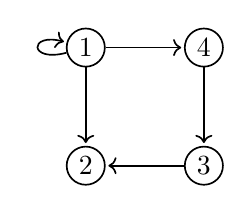
\begin{tikzpicture}[shorten >=1pt,node distance=1.5cm, semithick, on grid]
		\node[state, inner sep=2pt, minimum size=11pt]   (q_1)                {$1$};
		\node[state, inner sep=2pt, minimum size=11pt]   (q_2) [below=of q_1] {$2$};
		\node[state, inner sep=2pt, minimum size=11pt]   (q_3) [right=of q_2] {$3$};
		\node[state, inner sep=2pt, minimum size=11pt]   (q_4) [right=of q_1] {$4$};
		\path[->] (q_1) edge                node [above] {} (q_2)
		  			(q_3) edge                node [above] {} (q_2)
		  			(q_1) edge                node [above] {} (q_4)
		  			(q_4) edge                node [above] {} (q_3)
		(q_1) edge [loop left]    node [above] {} (q_1);
	\end{tikzpicture}
	\pause
	\begin{lstlisting}
edge(1,1).
edge(1,4).
edge(1,2).
edge(3,2).
edge(4,3).
	\end{lstlisting}
	\pause
	\begin{lstlisting}[firstnumber=7]
path(U, U).
path(U, W) :- edge(U, V), path(V, W).
	\end{lstlisting}
\end{frame}


\begin{frame} \frametitle{Aufgabe 1}
	\begin{minipage}{\dimexpr0.3\linewidth-\fboxrule-\fboxsep}
		\vfill
		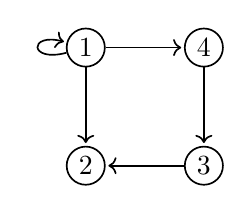
\begin{tikzpicture}[shorten >=1pt,node distance=1.5cm, semithick, on grid]
			\node[state, inner sep=2pt, minimum size=11pt]   (q_1)                {$1$};
			\node[state, inner sep=2pt, minimum size=11pt]   (q_2) [below=of q_1] {$2$};
			\node[state, inner sep=2pt, minimum size=11pt]   (q_3) [right=of q_2] {$3$};
			\node[state, inner sep=2pt, minimum size=11pt]   (q_4) [right=of q_1] {$4$};
			\path[->] (q_1) edge                node [above] {} (q_2)
			(q_3) edge                node [above] {} (q_2)
			(q_1) edge                node [above] {} (q_4)
			(q_4) edge                node [above] {} (q_3)
			(q_1) edge [loop left]    node [above] {} (q_1);
		\end{tikzpicture}
		\vfill
	\end{minipage}
	\begin{minipage}{\dimexpr0.49\linewidth-\fboxrule-\fboxsep}
		\footnotesize
		\begin{alignat*}{2}
			&\texttt{?- path(4,X).} \\
			\texttt{\{X=4\}} \quad &\texttt{?- .} && \texttt{\% 7 } \\[12pt]
			%
			&\texttt{?- path(4,X).}  \\
			&\texttt{?- edge(4,W), path(W,X).} \quad && \texttt{\% 8} \\
			\texttt{\{W=3\}} \quad &\texttt{?- path(3,X).} && \texttt{\% 5} \\
			\texttt{\{X=3\}} \quad &\texttt{?- .} && \texttt{\% 6}\\[12pt]
			%
			&\texttt{?- path(4,X).}  \\
			&\texttt{?- edge(4,W), path(W,X).} \quad && \texttt{\% 8} \\
			\texttt{\{W=3\}} \quad &\texttt{?- path(3,X).} && \texttt{\% 5} \\
			&\texttt{?- edge(3,U), path(U,X).} &&\texttt{\% 8} \\
			\texttt{\{U=2\}} \quad &\texttt{?- path(2,X).} &&\texttt{\% 4} \\
			\texttt{\{X=2\}} \quad &\texttt{?- .} &&\texttt{\% 7} \\
		\end{alignat*}
	\end{minipage}
\end{frame}


%%%%%%%%%%%%%%%%%%%%%%%%%%%%%%%%%%%%%%%%%%%%%%%%%%%%%%%%%%%%%%%%%%%%%%%%%%%%%%%%


\section{Aufgabe 2}

\begin{frame}[fragile] \frametitle{Aufgabe 2 -- Teil (a)}
	\begin{lstlisting}
nat(0).
nat(s(X)) :- nat(X).

sum(0, Y, Y) :- nat(Y).
sum(s(X), Y, s(S)) :- sum(X, Y, S).
	\end{lstlisting}
	
	\textbf{Gesucht:} Prädikat \texttt{even}, dass alle natürlichen Zahlen enthält
	
	\pause
	
	\begin{lstlisting}[firstnumber=7]
even(0).
even(s(s(N))) :- even(N).
	\end{lstlisting}
\end{frame}

\begin{frame}[fragile] \frametitle{Aufgabe 2 -- Teil (b)}
	\begin{lstlisting}
nat(0).
nat(s(X)) :- nat(X).

sum(0, Y, Y) :- nat(Y).
sum(s(X), Y, s(S)) :- sum(X, Y, S).

even(0).
even(s(s(N))) :- even(N).
	\end{lstlisting}
	
	\textbf{Gesucht:} Relation \texttt{div2} mit $(\num{\texttt{n}} , \num{\lfloor \frac{\texttt{n}}{\texttt{2}} \rfloor})$
	
	\pause
	
	\begin{lstlisting}[firstnumber=10]
div2(0, 0).
div2(s(0), 0).
div2(s(s(N)), s(M)) :- div2(N, M).
	\end{lstlisting}
\end{frame}

\begin{frame}[fragile] \frametitle{Aufgabe 2 -- Teil (c)}
	\begin{lstlisting}
nat(0).
nat(s(X)) :- nat(X).

sum(0, Y, Y) :- nat(Y).
sum(s(X), Y, s(S)) :- sum(X, Y, S).
	\end{lstlisting}
	
	\textbf{Gesucht:} Relation \texttt{div} mit $(\num{\texttt{n}} , \num{\texttt{m}} , \num{\lfloor \frac{\texttt{n}}{\texttt{m}} \rfloor})$
	
	\pause
	
	\begin{lstlisting}[firstnumber=14]
lt(0, s(M)) :- nat(M).
lt(s(N), s(M)) :- lt(N, M).
	\end{lstlisting}
	
	\pause
	
	\begin{lstlisting}[firstnumber=17]
div(0, M, 0) :- lt(0, M).
div(N, M, 0) :- lt(N, M).
div(N, M, s(Q)) :- lt(0, M), sum(M, V, N), 
                   div(V, M, Q).
	\end{lstlisting}
\end{frame}

\begin{frame} \frametitle{Aufgabe 2 -- Teil (d)}
	\scriptsize
	\begin{alignat*}{2}
		&\texttt{?- div(\num{3}, \num{2}, \num{1})} \\
		&\texttt{?- lt(\num{0}, \num{2}) , sum(\num{2}, V1, \num{3}) , div(V1, \num{2}, \num{0})} \qquad && \texttt{\% 19 } \\
		&\texttt{?- nat(\num{1}) , sum(\num{2}, V1, \num{3}) , div(V1, \num{2}, \num{0})}  && \texttt{\% 14} \\
		&\texttt{?- nat(\num{0}) , sum(\num{2}, V1, \num{3}) , div(V1, \num{2}, \num{0})} && \texttt{\% 2} \\
		&\texttt{?- sum(\num{2}, V1, \num{3}) , div(V1, \num{2}, \num{0}).} && \texttt{\% 1} \\
		&\texttt{?-* sum(\num{0}, V1, \num{1}) , div(V1, \num{2}, \num{0}).} && \texttt{\% 4} \\
		\texttt{\{V1=\num{1}\}} \quad &\texttt{?- nat(\num{1}) , div(\num{1}, \num{2}, \num{0}).} && \texttt{\% 3} \\
		&\texttt{?- nat(\num{0}) , div(\num{1}, \num{2}, \num{0}).} \quad && \texttt{\% 2} \\
		&\texttt{?- div(\num{1}, \num{2}, \num{0}).} && \texttt{\% 1} \\
		&\texttt{?- lt(\num{1}, \num{2}).} &&\texttt{\% 18} \\
		&\texttt{?- lt(\num{0}, \num{1}).} &&\texttt{\% 15} \\
		&\texttt{?- nat(\num{0}).} &&\texttt{\% 14} \\
		&\texttt{?- .} &&\texttt{\% 1} \\
	\end{alignat*}
\end{frame}

\end{document}

